% !TEX root = ../sommaire.tex

\chapter{Chapitre 4}

% !TEX root = ../sommaire.tex

\chapintro{En fait, j'en ai marre de mettre des résumés en anglais.}

%%%%%%%%%%%%%%%%%%%%%%%%%%%%%
\section{Section 1}
%%%%%%%%%%%%%%%%%%%%%%%%%%%%%

\begin{figure}
  \centering
  \subfigure[subfigure 1]{\label{fig:subfig1}
    \begin{tikzpicture}[scale = 1.5]
      \fill [black] (-1.25, -1.25) rectangle (1.25, 1.25); 
      \begin{scope}
        \clip (-1, -1) rectangle (0, 0);
        \fill[purple] (0,0) circle (1);
      \end{scope}
      \begin{scope}
        \clip (-1, 0) rectangle (0, 1);
        \fill[bleu] (0,0) circle (1);
      \end{scope}
      \begin{scope}
        \clip (0, 0) rectangle (1, 1);
        \fill[pink] (0,0) circle (1);
      \end{scope}
      \begin{scope}
        \clip (0, -1) rectangle (1, 0);
        \fill[vert] (0,0) circle (1);
      \end{scope}
    \end{tikzpicture}}
  \subfigure[subfigure 2]{\label{fig:subfig2}
    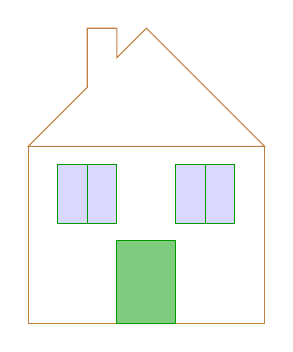
\begin{tikzpicture}[scale = 1.5]
      \draw[brown] (0, 0) -- (0.5, 0.5) -- (0.5, 1) -- (0.75, 1) -- (0.75, 0.75) -- (1, 1) -- (2, 0) -- cycle;
      \draw[brown] (0, 0) -- (0, -1.5) -- (2, -1.5) --  (2, 0);
      \draw[color = green!60!black, fill = blue, fill opacity = 0.15] (0.25, -0.65) rectangle (0.75, -0.15);
      \draw[color = green!60!black, fill = blue, fill opacity = 0.15] (1.25, -0.65) rectangle (1.75, -0.15);
      \draw[color = green!60!black] (0.5, -0.65) -- (0.5, -0.15);
      \draw[color = green!60!black] (1.5, -0.65) -- (1.5, -0.15);
      \filldraw[color = green!60!black, fill opacity = 0.5] (0.75, -1.5) rectangle (1.25, -0.8);
    \end{tikzpicture}}
  \subfigure[subfigure 3]{\label{fig:subfig3}
    
\includegraphics[scale = 0.3]{Pastry_Bag.png}
    }
  \caption[Dessins]{Subfigure 1 \ref{fig:subfig1} et subfigure 2 \ref{fig:subfig2}.}
  \label{fig:figure1}
\end{figure}

La figure \ref{fig:figure1} est vraiment magnifique. Elle est composée des sous-figures \ref{fig:subfig1}, \ref{fig:subfig2} et \ref{fig:subfig3}.

%%%%%%%%%%%%%%%%%%%%%%%%%%%%%
\section{Section 2}
%%%%%%%%%%%%%%%%%%%%%%%%%%%%%

\begin{algorithm}
  \begin{algorithmic}
    \STATE tableau d'entiers tab \COMMENT{tableau d'entiers}
    \STATE int $i$ \COMMENT{indice de parcours}
    \STATE int $m$ \COMMENT{valeur maximale du tableau}
    \STATE
    \STATE $m \leftarrow$ tab[1]
    \FOR{$i$ \FROM 2 \TO length(tab)}
      \IF{$m <$ tab[$i$]}
        \STATE $m \leftarrow$ tab[$i$]
      \ENDIF
      \STATE
      \STATE \PRINT "Le maximum est " + $m$
      \RETURN $m$
    \ENDFOR
  \end{algorithmic}
  \caption[Algorithme 1 (nom dans la liste des algorithmes)]{Met dans $m$ la valeur maximale du tableau tab.\label{ag:algo1}}
\end{algorithm}

L'algorithme \ref{ag:algo1} utilise le package \texttt{algorithmic} dont la francisation des termes se trouve dans le fichier \texttt{algo.sty}.

\begin{algorithm}
  \begin{C}
int max(int* tab, int n) {
  int i; // indice de parcours
  int m; // valeur maximale du tableau
  
  m = tab[0];
  for (i = 1; i < n; i++) {
    if (m < tab[i]) {
      m = tab[i];
    }
  }
  
  printf("Le maximum est %d", m),
  return m;
}
  \end{C}
  \caption[Algo en C]{Retourne la valeur maximale du tableau tab.\label{ag:algoc}}
\end{algorithm}

\begin{algorithm}
  \begin{PseudoCode}
max(tableau d'entiers tab, entier n) {
  entier i // indice de parcours
  entier m // valeur maximale du tableau
  
  m <- tab[1]
  for i from 2 to n {
    if (m < tab[i]) {
      m <- tab[i]
    }
  }
  
  print("Le maximum est ", m),
  return m;
}
  \end{PseudoCode}
  \caption[Algo en PseudoCode]{Retourne la valeur maximale du tableau tab.\label{ag:algop}}
\end{algorithm}

\begin{algorithm}
  \begin{Java}
int max(int[] tab, int n) {
  int i; // indice de parcours
  int m; // valeur maximale du tableau
  
  m = tab[0];
  for (i = 1; i < n; i++) {
    if (m < tab[i]) {
      m = tab[i];
    }
  }
  
  System.out.println("Le maximum est " + m),
  return m;
}
  \end{Java}
  \caption[Algo en Java]{Retourne la valeur maximale du tableau tab.\label{ag:algoj}}
\end{algorithm}

Les algorithmes \ref{ag:algoc} en C, \ref{ag:algop} en pseudo code, et \ref{ag:algoj} en Java utilisent le package \texttt{lstlistings}. La coloration sintaxique utilise les couleurs définies dans le fichier \texttt{couleurs.sty} et les mot-clés se trouvent dans le fichier \texttt{colorationSyntaxique.sty}. Vous pouvez modifier le fichier \texttt{colorationSyntaxique.sty} pour ajouter de nouveaux mot-clés ou y ajouter un langage, pour le moment seuls C, Java, Python, Shell, R et un pseudo code sont disponibles.

%%%%%%%%%%%%%%%%%%%%%%%%%%%%%
\section{Section 3}
%%%%%%%%%%%%%%%%%%%%%%%%%%%%%

La section 3.

%%%%%%%%%%%%%%%%%%%%%%%%%%%%%
\section{Conclusion}
%%%%%%%%%%%%%%%%%%%%%%%%%%%%%